\documentclass[a4paper]{article}
\usepackage[pdftex]{graphicx}
\usepackage[utf8]{inputenc}
\usepackage{enumerate}
\usepackage{amssymb}
\usepackage{colortbl}
\usepackage{icomma}
\usepackage{siunitx}
\sisetup{locale=DE} 
\usepackage{geometry}
\geometry{a4paper, top=15mm, left=15mm, right=15mm, bottom=15mm,
	headsep=10mm, footskip=12mm}
\usepackage{href-ul}
\hypersetup{
	colorlinks=true,
	linkcolor=blue,
	urlcolor=blue}
\usepackage{tikz}
\usetikzlibrary{positioning}
\usepackage{circuitikz}

\begin{document}
	
{\bf Verzweigte Stromkreise}
		
		
		\begin{enumerate}[1.]

	
		\begin{minipage}{0.75\textwidth}
				\item Du hast folgende Glühbirnen zur Auswahl: \\ Vervollständige die fehlenden technischen Daten!
				\vspace{0.5 cm}
				
			\renewcommand{\arraystretch}{2}
			\begin{tabular}{|c|c|c|c|c|}
				\hline
				& Spannung  U & Leistung P & Betriebsstromstärke I & Widerstand R \\ 
				\hline
			$L_1$	& 6 V  &  0,6 W & & \\
				\hline
			  $L_2$ & 6 V  & 1,8 W & & \\
				\hline
				$L_3$ & 3,5 V & 0,7 W & &   \\
				\hline
			\end{tabular}
		\end{minipage}	
		\begin{minipage}{0.2 \textwidth}
			
			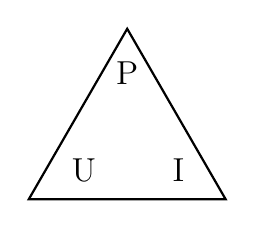
\begin{tikzpicture}[scale=1]
				% Dreieck mit Seitenlänge 2.5 cm
				\coordinate (U) at (0,0);
				\coordinate (I) at (2.5,0);
				\coordinate (P) at (1.25, {2.5*sqrt(3)/2});
				
				% Linien zeichnen
				\draw[thick] (U) -- (I) -- (P) -- cycle;
				
				% Beschriftung innerhalb
				\node[above=0.1cm of U, xshift=0.7cm] {\large U};
				\node[above=0.1cm of I, xshift=-0.6cm] {\large I};
				\node[below=0.3cm of P] {\large P};
			\end{tikzpicture}
			\vspace{0.5 cm}
			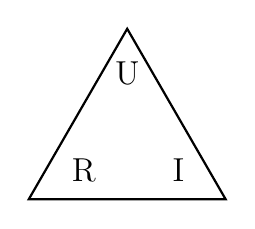
\begin{tikzpicture}[scale=1]
				% Dreieck mit Seitenlänge 2.5 cm
				\coordinate (R) at (0,0);
				\coordinate (I) at (2.5,0);
				\coordinate (U) at (1.25, {2.5*sqrt(3)/2});
				
				% Linien zeichnen
				\draw[thick] (R) -- (I) -- (U) -- cycle;
				
				% Beschriftung innerhalb
				\node[above=0.1cm of R, xshift=0.7cm] {\large R};
				\node[above=0.1cm of I, xshift=-0.6cm] {\large I};
				\node[below=0.3cm of U] {\large U};
			\end{tikzpicture}
		\end{minipage}			
		
	 Als Stromquelle dazu hast Du acht AAA 1,5 V Batterien, die Du in Reihe schalten kannst. 
	 \item Trage in die Stromkreise mögliche Kombinationen von Lampen und Stromquellen ein, sodass diese optimal leuchten!
	 Wie groß ist dann der Gesamtstrom? \\ 
	 Wieviele Batterien benutzt Du jeweils als Spannungsquelle?\\
	  Wie groß ist der Gesamtwiderstand der Schaltung? \\
	 

\begin{minipage}{0.5\textwidth} 
	 {\bf Schaltung A}
	 
	 \begin{circuitikz}[american]
	 	% Batterie (unten Negativ, oben Positiv), dann Reihe-Lampe L1,
	 	% dann Knoten mit zwei Lampen (L2 und L3) parallel, zurück zum Minus.
	 	\draw
	 	(0,0) node[ground]{}                       % Minus (Masse)
	 	to[battery1,l=$U$] (0,3)                   % Batterie
	 	to[lamp] (3,3) node (N){}           % Reihe-Lampe L1 und Knoten N
	 	-- (5,3)                                     % Verbindung zum oberen Verzweigungspunkt
	 	% erster paralleler Zweig (links)
	 	(3.5,3) to[lamp] (3.5,0) -- (0,0)
	 	% zweiter paralleler Zweig (rechts)
	 	(5,3)   to[lamp] (5,0)   -- (0,0)
	 	;
	 \end{circuitikz}
	 
	 \renewcommand{\arraystretch}{2}
	 \begin{tabular}{|p{1.6 cm}|p{1.6 cm}|p{1.6 cm}|p{1.6 cm}|}
	 	\hline
	 	$U_{ges}$ & $I_{ges}$ &  $R_{ges}$ & $P_{ges}$  \\ 
	 	\hline
	 	&  &  &  \\
	 	\hline
	 \end{tabular}
\end{minipage}			
\begin{minipage}{0.5\textwidth} 
	 {\bf Schaltung B}
	 
	 \begin{circuitikz}[american]
	 	% Batterie (unten Negativ, oben Positiv), dann Reihe-Lampe L1,
	 	% dann Knoten mit zwei Lampen (L2 und L3) parallel, zurück zum Minus.
	 	\draw
	 	(0,0) node[ground]{}                       % Minus (Masse)
	 	to[battery1,l=$U$] (0,3)                   % Batterie
	 	to[lamp] (3,3) node (N){}           % Reihe-Lampe L1 und Knoten N
	 	-- (6.5,3)                                     % Verbindung zum oberen Verzweigungspunkt
	 	% erster paralleler Zweig (links)
	 	(3.5,3) to[lamp] (3.5,0) -- (0,0)
	 	% zweiter paralleler Zweig (rechts)
	 	(5,3)   to[lamp] (5,0)   -- (0,0)
	 	% dritter paralleler Zweig (rechts)
	 	(6.5,3)   to[lamp] (6.5,0)   -- (0,0)
	 	;
	 \end{circuitikz}
	 
	 \renewcommand{\arraystretch}{2}
	 \begin{tabular}{|p{1.6 cm}|p{1.6 cm}|p{1.6 cm}|p{1.6 cm}|}
	 	\hline
	 	$U_{ges}$ & $I_{ges}$ &  $R_{ges}$ & $P_{ges}$  \\ 
	 	\hline
	 	&  &  &  \\
	 	\hline
	 \end{tabular}
\end{minipage}			
\vspace{0.5 cm}
	

\item Begründe, dass mit den gegebenen Lampen nur jeweils zwei gleiche Lampen in einer  Reihenschaltung Sinn machen.
\item Es werden nun {\bf zwei verschiedene Lampen in Reihe} geschaltet.
Beurteile für jede Kombination von Stromquelle und Lampen in der Tabelle, warum sie nicht sinnvoll ist und schildere Deine Beobachtung!

	\renewcommand{\arraystretch}{2}
\begin{tabular}{|c|c|p{12 cm}|}
	\hline
	Spannung  U & Kombination & Beobachtung  \\ 
	\hline
	3 V  &  $L_3$ + $L_1$  & \\
	\hline
	3 V  &  $L_3$ + $L_2$  & \\
	\hline
	4,5 V  &  $L_3$ + $L_2$  & \\
	\hline
	6 V  &  $L_3$ + $L_1$  & \\
	\hline
	6 V  &  $L_1$ + $L_2$  & \\
	\hline
\end{tabular}

\newpage 

\item Es werden nun {\bf zwei Lampen parallel} geschaltet
Beurteile für jede Kombination von Stromquelle und Lampen in der Tabelle, ob sie sinnvoll ist und schildere Deine Beobachtung!

\renewcommand{\arraystretch}{2}
\begin{tabular}{|c|c|p{12 cm}|}
	\hline
	Spannung  U & Kombination & Beobachtung  \\ 
	\hline
	3 V  &  $L_3$ + $L_3$  & \\
	\hline
	3 V  &  $L_3$ + $L_1$  & \\
	\hline
	3 V  &  $L_3$ + $L_2$  & \\
	\hline
	6 V  &  $L_1$ + $L_2$  & \\
	\hline
\end{tabular}

	\end{enumerate}
	
	\fbox{
		\begin{minipage}{0.5\textwidth}
		%	Zur Lösung bitte \href{https://www.okuyakl.de/phys/m/ll.pdf}{hier klicken} oder den QR-Code scannen.\\
			Weitere Arbeitsblätter gibt es unter 
			
			\href{https://www.okuyakl.de}{www.okuyakl.de}
		\end{minipage}
		\hfill
		\begin{minipage}{0.4\textwidth}
			\includegraphics[width=1.5 cm]{../../viecher/zwe03}
		%	\includegraphics[width=3 cm]{qr221}
			\includegraphics[width=2 cm]{../../viecher/afanticon1}
			
	\end{minipage}}
	
\end{document}